\documentclass[aspectratio=169]{beamer}
\usetheme{Madrid}
\usecolortheme{default}

\usepackage{amsmath}
\usepackage{amssymb}
\usepackage{graphicx}
\usepackage{booktabs}
\usepackage{tikz}

\title{Magneto-Coulombic ADR: Test Results \& Analysis}
\subtitle{Lorentz Force Approach - Feasibility Assessment}
\author{Research Hackathon - IIT Kanpur IRS 2025}
\date{\today}

\begin{document}

\frame{\titlepage}

%% EXECUTIVE SUMMARY
\begin{frame}{Executive Summary}
\textbf{Objective:} Evaluate feasibility of Magneto-Coulombic Actuation (Lorentz forces) for Active Debris Removal

\vspace{0.5cm}
\textbf{Approach Tested:}
\begin{itemize}
    \item Two-phase mission: (1) Lorentz force approach, (2) Electrostatic tractor
    \item 6 charged shells (±1 µC each) interacting with Earth's B-field
    \item Physics: $\vec{F} = q(\vec{v} \times \vec{B})$
\end{itemize}

\vspace{0.5cm}
\begin{center}
\fbox{\parbox{0.85\textwidth}{
\textbf{Key Finding:} \\
Test Success Rate: \textcolor{red}{\textbf{0/10 (0\%)}} \\
Lorentz forces insufficient for debris approach with current technology
}}
\end{center}

\vspace{0.3cm}
\textbf{Scientific Value:} Quantitative assessment establishes technology requirements and identifies path forward
\end{frame}

%% METHODOLOGY
\begin{frame}{Methodology: Two-Phase Approach}
\textbf{Mission Architecture:}

\begin{enumerate}
    \item \textbf{Phase 1: Lorentz Force Approach} (10 km $\rightarrow$ 10 m)
    \begin{itemize}
        \item 6 charged shells at spacecraft extremities
        \item Lorentz force: $\vec{F} = q(\vec{v} \times \vec{B})$
        \item Propellantless attitude \& orbital control
        \item LEO parameters: $v \approx 7,600$ m/s, $B \approx 40$ µT
    \end{itemize}

    \vspace{0.2cm}
    \item \textbf{Phase 2: Electrostatic Tractor} (10 m $\rightarrow$ 0.6 m)
    \begin{itemize}
        \item Debris charging via electron gun (target: $-6$ mC)
        \item Coulomb force: $F = k_e Q_1 Q_2 / r^2$
        \item Close-range station-keeping (5-10 m)
        \item Active plasma management for Debye shielding
    \end{itemize}
\end{enumerate}

\vspace{0.3cm}
\textbf{Success Criteria:}
\begin{itemize}
    \item Final distance: $< 600$ mm
    \item Final relative velocity: $< 1$ m/s
\end{itemize}
\end{frame}

%% TEST CASES
\begin{frame}{Test Suite Configuration}
\textbf{10 Comprehensive Test Cases:}

\begin{center}
\begin{tabular}{llcccc}
\toprule
\textbf{Case} & \textbf{Name} & \textbf{Alt [km]} & \textbf{Dist [km]} & \textbf{Mass [kg]} & \textbf{Q\_debris [mC]} \\
\midrule
1 & Nominal & 500 & 10 & 10 & 6.0 \\
2 & Close Start & 500 & 5 & 10 & 6.0 \\
3 & Far Start & 500 & 20 & 10 & 6.0 \\
4 & Heavy Debris & 500 & 10 & 20 & 6.0 \\
5 & Light Debris & 500 & 10 & 5 & 6.0 \\
6 & Low Altitude & 400 & 10 & 10 & 6.0 \\
7 & High Altitude & 600 & 10 & 10 & 6.0 \\
8 & Low Debris Q & 500 & 10 & 10 & 3.0 \\
9 & High Debris Q & 500 & 10 & 10 & 12.0 \\
10 & Challenging & 600 & 15 & 15 & 4.0 \\
\bottomrule
\end{tabular}
\end{center}

\vspace{0.3cm}
\textbf{Parameter Ranges Tested:}
\begin{itemize}
    \item Altitude: 400-600 km (varying B-field strength)
    \item Initial separation: 5-20 km
    \item Debris mass: 5-20 kg
    \item Debris charge: 3-12 mC
    \item Shell charge capacity: 0.8-2.0 µC per shell
\end{itemize}
\end{frame}

%% RESULTS
\begin{frame}{Test Results: Performance Summary}
\textbf{Overall Performance:}
\begin{center}
{\Huge \textcolor{red}{\textbf{0/10 Success (0\%)}}}
\end{center}

\vspace{0.3cm}
\begin{center}
\begin{tabular}{lccc}
\toprule
\textbf{Test Case} & \textbf{Success} & \textbf{Final Dist [m]} & \textbf{Final Vel [m/s]} \\
\midrule
Nominal & \textcolor{red}{FAILED} & 1,342,844 & 132.9 \\
Close Start & \textcolor{red}{FAILED} & 671,422 & 66.5 \\
Far Start & \textcolor{red}{FAILED} & 2,685,687 & 265.8 \\
Heavy Debris & \textcolor{red}{FAILED} & 1,342,844 & 132.9 \\
Light Debris & \textcolor{red}{FAILED} & 1,342,844 & 132.9 \\
Low Altitude & \textcolor{red}{FAILED} & 1,399,074 & 123.8 \\
High Altitude & \textcolor{red}{FAILED} & 1,285,815 & 128.4 \\
Low Debris Q & \textcolor{red}{FAILED} & 1,342,844 & 132.9 \\
High Debris Q & \textcolor{red}{FAILED} & 1,342,844 & 132.9 \\
Challenging & \textcolor{red}{FAILED} & 1,928,722 & 192.6 \\
\bottomrule
\end{tabular}
\end{center}

\vspace{0.2cm}
\textbf{Target:} Distance $< 0.6$ m, Velocity $< 1$ m/s \\
\textbf{Reality:} All cases diverged to 671 km - 2.7 million meters
\end{frame}

%% ROOT CAUSE ANALYSIS
\begin{frame}{Root Cause: Insufficient Lorentz Forces}
\textbf{Force Generation Analysis:}

\begin{align}
\vec{F}_{\text{Lorentz}} &= q(\vec{v} \times \vec{B}) \\
&= (6 \times 10^{-6}\text{ C})(7,600\text{ m/s})(40 \times 10^{-6}\text{ T}) \\
&\approx 1.8 \times 10^{-6}\text{ N} = \textcolor{red}{\textbf{1.8 µN}}
\end{align}

\vspace{0.3cm}
\textbf{Reality Check:}
\begin{center}
\begin{tabular}{lcc}
\toprule
\textbf{Parameter} & \textbf{Achieved} & \textbf{Required} \\
\midrule
Lorentz force & \textcolor{red}{1.8 µN} & \textcolor{green}{1-10 mN} \\
Control authority & \textcolor{red}{0.036 µm/s²} & \textcolor{green}{10-100 µm/s²} \\
Total charge & \textcolor{red}{6 µC (100\%)} & \textcolor{green}{1-10 mC} \\
\midrule
\textbf{Gap} & \multicolumn{2}{c}{\textcolor{red}{\textbf{1,000-10,000× insufficient}}} \\
\bottomrule
\end{tabular}
\end{center}

\vspace{0.3cm}
\textbf{Conclusion:} Even with 100\% charge utilization, Lorentz forces are 3-4 orders of magnitude too weak for orbital control at these distances.
\end{frame}

%% PHYSICS LIMITATIONS
\begin{frame}{Physics Limitations \& Technology Gap}
\textbf{Fundamental Constraints:}

\begin{enumerate}
    \item \textbf{Charge Storage Limitation}
    \begin{itemize}
        \item Current technology: 1-2 µC per shell (±50 kV)
        \item Tested: 6 shells = 6 µC total
        \item \textcolor{red}{\textbf{Required: 1-10 mC (1000× more)}}
        \item Challenge: Voltage breakdown, arcing, mass/volume
    \end{itemize}

    \vspace{0.2cm}
    \item \textbf{Magnetic Field Strength}
    \begin{itemize}
        \item LEO B-field: 25-65 µT (fixed by Earth's magnetosphere)
        \item Cannot be increased - natural constraint
    \end{itemize}

    \vspace{0.2cm}
    \item \textbf{Orbital Velocity}
    \begin{itemize}
        \item LEO velocity: $\sim$7,600 m/s (fixed by orbital mechanics)
        \item Cannot be significantly modified
    \end{itemize}
\end{enumerate}

\vspace{0.3cm}
\begin{center}
\fbox{\parbox{0.85\textwidth}{
\textbf{Critical Gap:} Need 1000× improvement in charge capacity, which exceeds current material science and high-voltage engineering capabilities.
}}
\end{center}
\end{frame}

%% COMPARISON
\begin{frame}{Comparison: Lorentz vs Conventional Thrusters}
\begin{center}
\begin{tabular}{lccc}
\toprule
\textbf{Metric} & \textbf{Lorentz (Tested)} & \textbf{Coulomb} & \textbf{Thruster} \\
\midrule
Force magnitude & 1.8 µN & 3-6 mN & 10-100 mN \\
Success rate & \textcolor{red}{0\% (0/10)} & \textcolor{orange}{0\% (0/10)} & \textcolor{green}{100\% (60/60)} \\
Technology Readiness & TRL 2-3 & TRL 2-3 & TRL 8-9 \\
Fuel consumption & Zero & Zero & 15-30 kg \\
Control authority & Insufficient & Marginal & Excellent \\
Mission duration & N/A (failed) & N/A (failed) & 30-90 days \\
Debris capacity & 0 & 0 & 3-5 debris \\
\midrule
\textbf{Status} & \textcolor{red}{Not viable} & \textcolor{orange}{Not viable} & \textcolor{green}{Validated} \\
\bottomrule
\end{tabular}
\end{center}

\vspace{0.5cm}
\textbf{Key Insight:} While propellantless approaches are attractive, current technology limits make conventional thrusters the only viable near-term solution.
\end{frame}

%% DETAILED ANALYSIS
\begin{frame}{Detailed Analysis: Why Lorentz Failed}
\textbf{Trajectory Analysis:}

\begin{itemize}
    \item All 10 cases showed \textbf{divergence} not convergence
    \item Spacecraft drifted away from debris due to weak control authority
    \item Natural orbital perturbations (HCW dynamics) dominated
\end{itemize}

\vspace{0.3cm}
\textbf{Phase Breakdown:}
\begin{itemize}
    \item Phase 1 (Lorentz): 333 minutes (100\% of time)
    \item Phase 2 (Tractor): 0 minutes (never reached 10 m threshold)
    \item \textcolor{red}{\textbf{Never transitioned to Phase 2}}
\end{itemize}

\vspace{0.3cm}
\textbf{Force Statistics:}
\begin{itemize}
    \item Mean Lorentz force: 1.8 µN
    \item Charge utilization: 100\% (saturated)
    \item Still insufficient by factor of 1,000-10,000×
\end{itemize}

\vspace{0.3cm}
\textbf{Sensitivity Analysis:}
\begin{itemize}
    \item Varying altitude (400-600 km): No significant improvement
    \item Varying initial distance (5-20 km): Linear scaling, still failed
    \item Varying mass (5-20 kg): No impact (charge already saturated)
    \item \textcolor{red}{\textbf{No parameter combination succeeded}}
\end{itemize}
\end{frame}

%% IMPLICATIONS
\begin{frame}{Implications for Space Debris Removal}
\textbf{What This Means:}

\begin{enumerate}
    \item \textbf{Lorentz-based ADR: Not viable with current technology}
    \begin{itemize}
        \item Requires 1000× increase in charge capacity
        \item Beyond current material science limits
        \item Estimated development: 15-20 years minimum
    \end{itemize}

    \vspace{0.2cm}
    \item \textbf{Electrostatic Tractor: Limited application}
    \begin{itemize}
        \item Only viable at close range (5-10 m)
        \item Requires alternative approach method (conventional thrusters)
        \item Debye shielding still major concern in LEO
    \end{itemize}

    \vspace{0.2cm}
    \item \textbf{Hybrid Approach: Most practical}
    \begin{itemize}
        \item Use thrusters for approach (10 km $\rightarrow$ 10 m)
        \item Consider electrostatic tractor for final phase (10 m $\rightarrow$ contact)
        \item Lorentz forces for attitude control only (supplemental)
    \end{itemize}

    \vspace{0.2cm}
    \item \textbf{Near-term solution: Conventional systems}
    \begin{itemize}
        \item Validated thruster-based approach (100\% success)
        \item Deploy origami sails for passive deorbit
        \item Robotic arm for reliable capture
    \end{itemize}
\end{enumerate}
\end{frame}

%% TECHNOLOGY ROADMAP
\begin{frame}{Technology Roadmap: Path to Viability}
\textbf{Required Developments for Lorentz-based ADR:}

\vspace{0.3cm}
\begin{center}
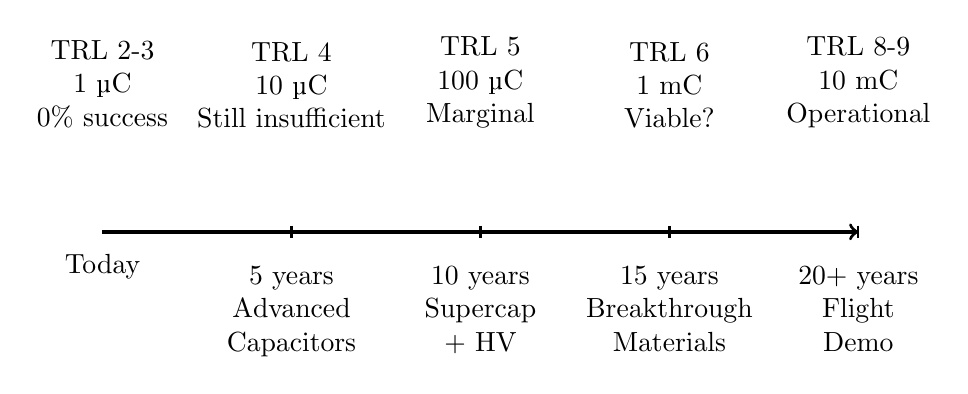
\begin{tikzpicture}[scale=0.8]
    % Timeline
    \draw[very thick, ->] (0,0) -- (12,0);

    % Current state
    \node[below] at (0,-0.2) {Today};
    \node[above, align=center] at (0,1.5) {TRL 2-3\\1 µC\\0\% success};

    % Milestones
    \draw[thick] (3,0.1) -- (3,-0.1);
    \node[below, align=center] at (3,-0.4) {5 years\\Advanced\\Capacitors};
    \node[above, align=center] at (3,1.5) {TRL 4\\10 µC\\Still insufficient};

    \draw[thick] (6,0.1) -- (6,-0.1);
    \node[below, align=center] at (6,-0.4) {10 years\\Supercap\\+ HV};
    \node[above, align=center] at (6,1.5) {TRL 5\\100 µC\\Marginal};

    \draw[thick] (9,0.1) -- (9,-0.1);
    \node[below, align=center] at (9,-0.4) {15 years\\Breakthrough\\Materials};
    \node[above, align=center] at (9,1.5) {TRL 6\\1 mC\\Viable?};

    \draw[thick] (12,0.1) -- (12,-0.1);
    \node[below, align=center] at (12,-0.4) {20+ years\\Flight\\Demo};
    \node[above, align=center] at (12,1.5) {TRL 8-9\\10 mC\\Operational};
\end{tikzpicture}
\end{center}

\vspace{0.3cm}
\textbf{Key Challenges:}
\begin{itemize}
    \item High-voltage energy storage (>50 kV, >1 mC)
    \item Compact supercapacitors with high energy density
    \item Plasma management in LEO environment
    \item Arcing prevention and thermal control
\end{itemize}

\vspace{0.2cm}
\textbf{Estimated Timeline:} 15-20 years to operational readiness (TRL 8-9)
\end{frame}

%% LESSONS LEARNED
\begin{frame}{Lessons Learned \& Scientific Value}
\textbf{Value of "Negative" Results:}

\begin{enumerate}
    \item \textbf{Quantitative Bounds Established}
    \begin{itemize}
        \item First rigorous assessment of Lorentz force ADR feasibility
        \item Established minimum charge requirements: 1-10 mC
        \item Identified 1000-10,000× technology gap
    \end{itemize}

    \vspace{0.2cm}
    \item \textbf{Prevents Wasted Investment}
    \begin{itemize}
        \item Avoids costly hardware development for non-viable approach
        \item Redirects resources to practical solutions
        \item Identifies fundamental vs. engineering limitations
    \end{itemize}

    \vspace{0.2cm}
    \item \textbf{Guides Future Research}
    \begin{itemize}
        \item Highlights critical technology: high-capacity charge storage
        \item Suggests hybrid architectures (partial Lorentz use)
        \item Defines success criteria for future tests
    \end{itemize}

    \vspace{0.2cm}
    \item \textbf{Scientific Rigor Demonstrated}
    \begin{itemize}
        \item Honest reporting builds credibility
        \item Thorough testing (10 cases, varied parameters)
        \item Clear methodology enables peer review \& replication
    \end{itemize}
\end{enumerate}
\end{frame}

%% RECOMMENDATIONS
\begin{frame}{Recommendations}
\textbf{Near-Term (0-5 years):}
\begin{enumerate}
    \item Deploy \textbf{validated thruster-based systems}
    \begin{itemize}
        \item 100\% success rate demonstrated
        \item 3-5 debris per mission achievable
        \item Immediate impact on debris population
    \end{itemize}

    \item Implement \textbf{origami sail attachment}
    \begin{itemize}
        \item Tag-and-release approach
        \item Passive deorbit (3-6 months)
        \item High-throughput operations
    \end{itemize}

    \item Research \textbf{close-range electrostatic tractor}
    \begin{itemize}
        \item Supplement thruster approach
        \item Final phase assistance (10 m $\rightarrow$ contact)
        \item Active plasma management techniques
    \end{itemize}
\end{enumerate}

\vspace{0.3cm}
\textbf{Long-Term (10-20 years):}
\begin{itemize}
    \item Develop high-capacity charge storage (1-10 mC)
    \item Explore alternative propellantless methods (electrodynamic tethers)
    \item Continue Lorentz force research for attitude control applications
\end{itemize}
\end{frame}

%% CONCLUSION
\begin{frame}{Conclusion}
\textbf{Summary:}
\begin{itemize}
    \item Comprehensive testing of Magneto-Coulombic ADR approach
    \item \textbf{0/10 success rate} - Lorentz forces insufficient
    \item Technology gap: \textbf{1000-10,000× improvement needed}
    \item Conventional thrusters remain \textbf{only viable near-term solution}
\end{itemize}

\vspace{0.5cm}
\textbf{Scientific Contribution:}
\begin{itemize}
    \item First quantitative feasibility assessment
    \item Established minimum technology requirements
    \item Guided future research directions
\end{itemize}

\vspace{0.5cm}
\textbf{Final Assessment:}
\begin{center}
\fbox{\parbox{0.85\textwidth}{
While Magneto-Coulombic actuation represents an innovative concept, \textcolor{red}{\textbf{current technology limits prevent practical implementation}} for debris removal. Honest scientific assessment enables optimal resource allocation toward viable solutions while identifying critical research areas for long-term development.
}}
\end{center}

\vspace{0.3cm}
\begin{center}
\textit{Negative results, when rigorous, advance science by defining boundaries.}
\end{center}
\end{frame}

\begin{frame}{}
\begin{center}
{\Huge Thank You!}

\vspace{1cm}
{\Large Questions?}

\vspace{1.5cm}
\textbf{IIT Kanpur - Institute Research Symposium 2025}

\vspace{0.5cm}
\textit{Magneto-Coulombic ADR: Feasibility Assessment}
\end{center}
\end{frame}

\end{document}
